\section{Planning}

The bounds discussed in \cref{sec:bounds} have applications in various contexts, both for POMDPs and other domains. In this section, we examine how these bounds can be effectively employed in belief space planning. We start with general formulations of bounds for POMDPs. Subsequently, we focus on information-theoretic rewards, particularly entropy. Finally, we address the challenges of planning in high-dimensional state spaces.

\subsection{Reward and Value Functions}

In the context of planning, the general reward function is denoted as $\reward{\blf{},\pi,\blf{}^\prime}$. Our goal in planning is to bound the cumulative expected reward, as represented in \eqref{eq:value_function}, where the expectation is explicitly given on observations and implicitly for states in the reward structure. By reducing the domain over which this expectation is calculated ---whether with respect to states, observations, or both--- we can achieve improved computational efficiency (see \cref{sec:complexity}) while providing formal performance guarantees. In this paper we focus on bounding the expectation with respect to the observations, although similar bounds can be formulated for the state space.

We begin by bounding the expected reward with respect to the observation space:
\begin{equation}
		\expectation{\reward{\blf{},\pi}}{\observationsRV{}}-\partialexpectation{\reward{\blf{},\pi(\blf{})}}{\subSpaceI{\observations{}}}
		\leq\measure{\stcompI{\subSpace}{\observations{}}}\sup_{\observations{}\in\stcompI{\subSpace}{\observations{}}}\reward{\blf{},\pi(\blf{})}\;,
\end{equation}
where $\subSpaceI{\observations{}}\subseteq\observationSpace$.

In many planning scenarios, the belief dependent reward is assumed to have a structure of $\reward{\blf{},\pi(\blf{})}\equiv \expectation{R(\blf{}(\statesRV{}),\statesRV{},\pi(\blf{}))}{\statesRV{}\sim\blf{}}$. For such cases, we can derive bounds on the reward with respect to the state space:
\begin{equation}
		\expectation{R(\blf{}(\statesRV{}),\statesRV{},\pi(\blf{}))}{\statesRV{}\sim\blf{}}-\partialexpectation{R(\blf{}(\statesRV{}),\statesRV{},\pi(\blf{}))}{\subSpaceI{\states{}}}
		\leq\measure{\stcompI{\subSpace}{\states{}}}\sup_{\states{}\in\stcompI{\subSpace}{\states{}}}R(\blf{}(\states{}),\states{},\pi(\blf{}))\;,
\end{equation}
where $\subSpaceI{\states{}}\subseteq\stateSpace$.

Not all rewards depend on the belief. State-dependent rewards, given by $\expectation{R(\statesRV{},\pi(\blf{}))}{\statesRV{}\sim\blf{}}$, follow a similar pattern but often benefit from known $R_{\min}$ and $R_{\max}$ values, simplifying the bounds to:
\begin{equation}
	\begin{split}
		\expectation{R(\statesRV{},\pi(\blf{}))}{\statesRV{}\sim\blf{}}-\partialexpectation{R(\statesRV{},\pi(\blf{}))}{\subSpaceI{\states{}}}&\leq\measure{\stcompI{\subSpace}{\states{}}}\sup_{\states{}\in\stcompI{\subSpace}{\states{}}}R(\states{},\pi(\blf{}))             \\
		 &\leq\measure{\stcompI{\subSpace}{\states{}}}R_{\max}\;.
	\end{split}
\end{equation}
If we further look at action sequences and not policies, then the case of state dependent rewards further simplifies matters by being independent of the observations.

These bounds can be jointly used to reduce the computational complexity by reducing the state and observation spaces concurrently.

With these reward bounds, we can proceed to bound the value function. When bounding with respect to the state space:
\begin{corollaryE}[][end, no link to proof]
	\label{thm:val_func_bounds_states}
	$\lowerbound^\pi(\blf{k})\leq V^\pi(\blf{k})-\bar{V}^\pi(\blf{k})\leq\upperbound^\pi(\blf{k})$, where:
	\begin{subequations}
		\begin{align}
			\lowerbound\nolimits^\pi(\blf{k})& =\measure{\stcompI{\subSpace}{k}}\inf_{\states{k}\in\stcompI{\subSpace}{k}}R_k+\sum_{l=k+1}^{k+L}\gamma^{l-k}\expectation{\measure{\stcompI{\subSpace}{l}}\inf_{\states{l}\in\stcompI{\subSpace}{l}}\boldsymbol{R}_l}{\observationsRV{k+1:l}}\;,\\
			\upperbound\nolimits^\pi(\blf{k}) & =\measure{\stcompI{\subSpace}{k}}\sup_{\states{k}\in\stcompI{\subSpace}{k}}R_k+\sum_{l=k+1}^{k+L}\gamma^{l-k}\expectation{\measure{\stcompI{\subSpace}{l}}\sup_{\states{l}\in\stcompI{\subSpace}{l}}\boldsymbol{R}_l}{\observationsRV{k+1:l}}\;,\\
			\bar{V}^\pi(\blf{k}) & =\partialexpectation{\boldsymbol{R}_k}{\subSpaceI{k}}+\sum_{l=k+1}^{k+L}\gamma^{l-k}\expectation{\partialexpectation{\boldsymbol{R}_l}{\subSpaceI{l}}}{\observationsRV{k+1:l}}\;.
		\end{align}
	\end{subequations}
	and $R_k\triangleq R(\blf{k}(\states{k}),\states{k},\pi(\blf{k}))$.
\end{corollaryE}
\begin{proofE}
	Applying \cref{thm:general_bounds} to $\expectation{\boldsymbol{R}_l}{\states{l}}$ and summing for the cumulative reward results in the desired bounds.
\end{proofE}
\noindent We use the shorthand $R_k\triangleq R(\blf{k}(\states{k}),\states{k},\pi(\blf{k}))$.

Expressing the bounds in a recursive manner, as is done for the value function with the bellman equation \eqref{eq:bellman}, we find the following:
\begin{corollaryE}[][end, no link to proof]
	\label{thm:val_func_bounds_states_bellman}
	$\lowerbound^\pi(\blf{t})\leq V^\pi(\blf{t})-\bar{V}^\pi(\blf{t})\leq\upperbound^\pi(\blf{t})\quad\forall t\in[k,k+L]$, where:
	\begin{subequations}
		\begin{align}
			\lowerbound\nolimits^\pi(\blf{t}) & =\measure{\stcompI{\subSpace}{t}}\inf_{\states{t}\in\stcompI{\subSpace}{t}}R_t+\gamma\expectation{\lowerbound(\blf{t+1})}{\observationsRV{t+1}}\;,\\
			\upperbound\nolimits^\pi(\blf{t}) & =\measure{\stcompI{\subSpace}{t}}\sup_{\states{t}\in\stcompI{\subSpace}{t}}R_t+\gamma\expectation{\upperbound(\blf{t+1})}{\observationsRV{t+1}}\;,\\
			\bar{V}^\pi(\blf{t}) & =\partialexpectation{\boldsymbol{R}_t}{\subSpaceI{t}}
			+\gamma\expectation{\bar{V}^\pi(\blf{t+1})}{\observationsRV{t+1}}\;.
		\end{align}
	\end{subequations}
	and $\lowerbound^\pi(\blf{k+L})=\upperbound^\pi(\blf{k+L})=V^\pi(\blf{k+L})=\bar{V}^\pi(\blf{k+L})=0$, $\subSpaceI{t}\subseteq\stateSpace$.
\end{corollaryE}
\begin{proofE}
	Proof by induction:

	\textbf{\underline{base case:}}
	\begin{align*}
		\upperbound\nolimits^\pi(\blf{k+L-1})&=\measure{\stcompI{\subSpace}{k+L-1}}\sup_{\states{k+L-1}\in\stcompI{\subSpace}{k+L-1}}R_t+\gamma\expectation{\upperbound(\blf{k+L})}{\observationsRV{k+L}}\\
		&=\measure{\stcompI{\subSpace}{k+L-1}}\sup_{\states{k+L-1}\in\stcompI{\subSpace}{k+L-1}}R_t\;,\\
		\bar{V}^\pi(\blf{k+L-1}) & =\partialexpectation{\boldsymbol{R}_t}{\subSpaceI{k+L-1}}
		+\gamma\expectation{\bar{V}^\pi(\blf{k+L})}{\observationsRV{k+L}}\\
		&=\partialexpectation{\boldsymbol{R}_{k+L-1}}{\subSpaceI{k+L-1}}\;,\\
		V^\pi(\blf{k+L-1})&=\expectation{\boldsymbol{R}_{k+L-1}}{\statesRV{k+L-1}}
		+\gamma\expectation{V^\pi(\blf{k+L})}{\observationsRV{k+L}}\\
		&=\expectation{\boldsymbol{R}_{k+L-1}}{\statesRV{k+L-1}}\;.
	\end{align*}
	Put together we find that the inequality holds as it is a direct consequence of \cref{thm:general_bounds} for $\expectation{\boldsymbol{R}_{k+L-1}}{\statesRV{k+L-1}}$.

	\textbf{\underline{induction step:}}
	Let us assume that $V^\pi(\blf{t+1})-\bar{V}^\pi(\blf{t+1})\leq\upperbound(\blf{t+1})$ then
	\begin{align*}
		V^\pi(\blf{t})&-\bar{V}^\pi(\blf{t})\\
		\begin{split}
			&=\expectation{R(\blf{t}(\statesRV{t}),\statesRV{t},\pi(\blf{t}))}{\statesRV{t}}-\partialexpectation{R(\blf{t}(\statesRV{t}),\statesRV{t},\pi(\blf{t}))}{\subSpaceI{t}} \\
			&\phantomeq+\gamma\left(\expectation{V^\pi(\blf{t+1})-\bar{V}^\pi(\blf{t+1})}{\observationsRV{t+1}}\right)
		\end{split}    \\
		\begin{split}
			&\leq\expectation{R(\blf{t}(\statesRV{t}),\statesRV{t},\pi(\blf{t}))}{\statesRV{t}}-\partialexpectation{R(\blf{t}(\statesRV{t}),\statesRV{t},\pi(\blf{t}))}{\subSpaceI{t}} \\
			&\phantomeq+\gamma\left(\expectation{\upperbound(\blf{t+1})}{\observationsRV{t+1}}\right)
		\end{split} \\
		&\leq\measure{\subSpaceI{t+1}}\sup_{\stcompI{\subSpace}{t+1}}R(\blf{t}(\statesRV{t}),\statesRV{t},\pi(\blf{t}))+\gamma\left(\expectation{\upperbound(\blf{t+1})}{\observationsRV{t+1}}\right)\qed
	\end{align*}
\end{proofE}

As was done for the reward, we can also bound with respect to the observation space:
\begin{corollaryE}[][end, no link to proof]
	\label{thm:val_func_bounds_obs}
	$\lowerbound^\pi(\blf{k})\leq V^\pi(\blf{k})-\bar{V}^\pi(\blf{k})\leq\upperbound^\pi(\blf{k})$, where:
	\begin{small}
		\begin{subequations}
			\begin{align}
				\lowerbound\nolimits^\pi(\blf{k})& =\sum_{l=k}^{k+L-1}\gamma^{l-k}\measure{\stcompI{\subSpace}{k+1:l+1}\mid\blf{k},\pi}\inf_{\observations{k+1:l+1}\in\stcompI{\subSpace}{k+1:l+1}}\reward{\blf{l},\pi_l,\blf{l+1}}\;, \\
				\upperbound\nolimits^\pi(\blf{k})& =\sum_{l=k}^{k+L-1}\gamma^{l-k}\measure{\stcompI{\subSpace}{k+1:l+1}\mid\blf{k},\pi}\sup_{\observations{k+1:l+1}\in\stcompI{\subSpace}{k+1:l+1}}\reward{\blf{l},\pi_l,\blf{l+1}}\;, \\
				\bar{V}^\pi(\blf{k}) & =\sum_{l=k}^{k+L-1}\gamma^{l-k}\partialexpectation{\reward{\blf{l},\pi_l,\blf{l+1}}}{\subSpaceI{k+1:l+1}\mid\blf{k},\pi}\;,
			\end{align}
		\end{subequations}
	\end{small}
	and $\subSpaceI{k+1:l+1}\subseteq\observationSpace^{l-k}$ which is the joint observation space over time.
\end{corollaryE}
\begin{proofE}
	Beginning with \eqref{eq:value_function} we look for bounds on $\expectation{\reward{\blf{l},\pi_l,\blf{l+1}}}{\observationsRV{k+1:l+1}\mid\blf{k},\pi}$. Applying \cref{thm:general_bounds} leads us directly to the bounds for a single time step. Subsequently we sum over all time-steps.
\end{proofE}

If we wish to propagate the choice of subset not just to the immediate expected reward, but through to the entire value function, thus completely eliminating specific realizations of observations from the objective function, we find:
\begin{corollaryE}[][end, no link to proof]
	\label{thm:val_func_bounds_obs_bellman}
	$\lowerbound^\pi(\blf{t})\leq V^\pi(\blf{t})-\bar{V}^\pi(\blf{t})\leq\upperbound^\pi(\blf{t})\quad\forall t\in[k,k+L]$, where:
	\begin{small}
		\begin{subequations}
			\begin{align}
				\begin{split}
					\lowerbound\nolimits^\pi(\blf{t})&=\measure{\stcompI{\subSpace}{t+1}\mid\blf{t},\pi}\Bigl(\inf_{\stcompI{\subSpace}{t+1}}\reward{\blf{t},\pi_t,\blf{t+1}}+\gamma\inf_{\stcompI{\subSpace}{t+1}}\bar{V}^\pi(\blf{t+1})\Bigr)\\
					&+
					\gamma\Bigl(\measure{\stcompI{\subSpace}{t+1}\mid\blf{t},\pi}\inf_{\stcompI{\subSpace}{t+1}}\lowerbound(\blf{t+1})+\partialexpectation{\lowerbound(\blf{t+1})}{\subSpaceI{t+1}\mid\blf{t},\pi}\Bigr)\;,
				\end{split}\\
				\begin{split}
					\upperbound\nolimits^\pi(\blf{t})&=\measure{\stcompI{\subSpace}{t+1}\mid\blf{t},\pi}\Bigl(\sup_{\stcompI{\subSpace}{t+1}}\reward{\blf{t},\pi_t,\blf{t+1}}+\gamma\sup_{\stcompI{\subSpace}{t+1}}\bar{V}^\pi(\blf{t+1})\Bigr)\\
					&+
					\gamma\Bigl(\measure{\stcompI{\subSpace}{t+1}\mid\blf{t},\pi}\sup_{\stcompI{\subSpace}{t+1}}\lowerbound(\blf{t+1})+\partialexpectation{\lowerbound(\blf{t+1})}{\subSpaceI{t+1}\mid\blf{t},\pi}\Bigr)\;,
				\end{split}\\
				\bar{V}^\pi(\blf{t}) &=\partialexpectation{\reward{\blf{t},\pi_t,\blf{t+1}}}{\subSpaceI{t+1}\mid\blf{t},\pi}+\gamma\partialexpectation{\bar{V}^\pi(\blf{t+1})}{\subSpaceI{t+1}\mid\blf{t},\pi}\;,
			\end{align}
		\end{subequations}
	\end{small}
	and $\lowerbound^\pi(\blf{k+L})=\upperbound^\pi(\blf{k+L})=V^\pi(\blf{k+L})=\bar{V}^\pi(\blf{k+L})=0$ and $\subSpaceI{t}\subseteq\observationSpace$.
\end{corollaryE}
\begin{proofE}
	Proof by induction:

	\textbf{\underline{base case:}}
	\begin{align*}
		\upperbound\nolimits^\pi(\blf{k+L-1})&=\measure{\stcompI{\subSpace}{k+L}\mid\blf{k+L-1},\pi}\Bigl(\sup_{\stcompI{\subSpace}{k+L}}\reward{\blf{k+L-1},\pi_t,\blf{k+L}}+\gamma\sup_{\stcompI{\subSpace}{k+L}}\bar{V}^\pi(\blf{k+L})\Bigr)\\
		&+
		\gamma\Bigl(\measure{\stcompI{\subSpace}{k+L}\mid\blf{t},\pi}\sup_{\stcompI{\subSpace}{k+L}}\lowerbound(\blf{k+L})+\partialexpectation{\lowerbound(\blf{k+L})}{\subSpaceI{k+L}\mid\blf{k+L-1},\pi}\Bigr)\\
		&=\measure{\stcompI{\subSpace}{k+L}\mid\blf{k+L-1},\pi}\Bigl(\sup_{\stcompI{\subSpace}{k+L}}\reward{\blf{k+L-1},\pi_t,\blf{k+L}}\Bigr)\;,\\
		\bar{V}^\pi(\blf{k+L-1}) &=\partialexpectation{\reward{\blf{k+L-1},\pi_{k+L-1},\blf{k+L}}}{\subSpaceI{k+L}\mid\blf{k+L-1},\pi}+\gamma\partialexpectation{\bar{V}^\pi(\blf{k+L})}{\subSpaceI{k+L}\mid\blf{k+L-1},\pi}\\
		&=\partialexpectation{\reward{\blf{k+L-1},\pi_{k+L-1},\blf{k+L}}}{\subSpaceI{k+L}\mid\blf{k+L-1},\pi}\;,\\
		V^\pi(\blf{k+L-1})&=\expectation{\reward{\blf{k+L-1},\pi_{k+L-1},\blf{k+L}}}{\observationsRV{k+L}\mid\blf{k+L-1},\pi}+\gamma\expectation{V^\pi(\blf{k+L})}{\observationsRV{k+L}}\\
		&=\expectation{\reward{\blf{k+L-1},\pi_{k+L-1},\blf{k+L}}}{\observationsRV{k+L}\mid\blf{k+L-1},\pi}\;.
	\end{align*}
	Put together we find that the inequality holds as it is a direct consequence of \cref{thm:general_bounds} for $\expectation{\reward{\blf{k+L-1},\pi_{k+L-1},\blf{k+L}}}{\observationsRV{k+L}\mid\blf{k+L-1},\pi}$.

	\textbf{\underline{induction step:}}
	, let us assume that $V^\pi(\blf{t+1})-\bar{V}^\pi(\blf{t+1})\leq\upperbound(\blf{t+1})$ then
	\begin{align*}
		V^\pi(\blf{t})&-\bar{V}^\pi(\blf{t})\\
		\begin{split}
			=&\expectation{\reward{\blf{t},\pi_t,\blf{t+1}}}{\observationsRV{t+1}}-\partialexpectation{\reward{\blf{t},\pi_t,\blf{t+1}}}{\subSpaceI{t+1}}\\
			&+\gamma\left(\expectation{V^\pi(\blf{t+1})}{\observationsRV{t+1}}-\partialexpectation{\bar{V}^\pi(\blf{t+1})}{\subSpaceI{t+1}}\right)
		\end{split}\\
		\begin{split}
			\leq&\measure{\stcompI{\subSpace}{t+1}}\sup_{\stcompI{\subSpace}{t+1}}\reward{\blf{t},\pi_t,\blf{t+1}}\\
			&+\partialexpectation{\reward{\blf{t},\pi_t,\blf{t+1}}}{\subSpaceI{t+1}}-\partialexpectation{\reward{\blf{t},\pi_t,\blf{t+1}}}{\subSpaceI{t+1}}\\
			&+\gamma\measure{\stcompI{\subSpace}{t+1}}\sup_{\stcompI{\subSpace}{t+1}}V^\pi(\blf{t+1})+\gamma\left(\partialexpectation{V^\pi(\blf{t+1})}{\subSpaceI{t+1}}-\partialexpectation{\bar{V}^\pi(\blf{t+1})}{\subSpaceI{t+1}}\right)
		\end{split}\\
		\begin{split}
			\leq&\measure{\stcompI{\subSpace}{t+1}}\sup_{\stcompI{\subSpace}{t+1}}\reward{\blf{t},\pi_t,\blf{t+1}}\\
			&+\gamma\left(\measure{\stcompI{\subSpace}{t+1}}\sup_{\stcompI{\subSpace}{t+1}}V^\pi(\blf{t+1})+\partialexpectation{\upperbound(\blf{t+1})}{\subSpaceI{t+1}}\right)
		\end{split}\\
		\begin{split}
			=&\measure{\stcompI{\subSpace}{t+1}}\sup_{\stcompI{\subSpace}{t+1}}\reward{\blf{t},\pi_t,\blf{t+1}}\\
			&+\gamma\measure{\stcompI{\subSpace}{t+1}}\sup_{\stcompI{\subSpace}{t+1}}\left(V^\pi(\blf{t+1})-\bar{V}^\pi(\blf{t+1})+\bar{V}^\pi(\blf{t+1})\right) \\
			&+\gamma\partialexpectation{\upperbound(\blf{t+1})}{\subSpaceI{t+1}}
		\end{split}\\
		\begin{split}
			\leq&\measure{\stcompI{\subSpace}{t+1}}\sup_{\stcompI{\subSpace}{t+1}}\reward{\blf{t},\pi_t,\blf{t+1}}\\
			&+\gamma\measure{\stcompI{\subSpace}{t+1}}\sup_{\stcompI{\subSpace}{t+1}}\left(\upperbound(\blf{t+1})+\bar{V}^\pi(\blf{t+1})\right)+\gamma\partialexpectation{\upperbound(\blf{t+1})}{\subSpaceI{t+1}}
		\end{split}\\
		\begin{split}
			\leq&\measure{\stcompI{\subSpace}{t+1}}\sup_{\stcompI{\subSpace}{t+1}}\reward{\blf{t},\pi_t,\blf{t+1}}\\
			&+\gamma\measure{\stcompI{\subSpace}{t+1}}\left(\sup_{\stcompI{\subSpace}{t+1}}\upperbound(\blf{t+1})+\sup_{\stcompI{\subSpace}{t+1}}\bar{V}^\pi(\blf{t+1})\right)+\gamma\partialexpectation{\upperbound(\blf{t+1})}{\subSpaceI{t+1}}\qed
		\end{split}
	\end{align*}
\end{proofE}

In \cref{thm:val_func_bounds_obs_bellman} the choice of subsets $\subSpaceI{t}$ is used for bounding the expected reward as well as the cumulative expected rewards. If one were to construct a belief tree, then the choice of subset would be analogous to pruning the branches indicated by $\stcomp{\subSpace}$.

An alternative approach which proves to be more manageable to formulate is to take the partial expectation only with respect to the immediate expected reward. This approach still allows for closed-loop planning, but does not prune the tree, instead it simplifies calculations for the immediate expected reward.
\begin{corollaryE}[][end, no link to proof]
	\label{thm:val_func_immediate_bounds_obs_bellman}
	$\lowerbound(\blf{t})\leq V^\pi(\blf{t})-\bar{V}^\pi(\blf{t})\leq\upperbound(\blf{t})\quad\forall t\in[k,k+L]$, where:
	\begin{small}
		\begin{subequations}
			\begin{align}
				\lowerbound(\blf{t}) & =\measure{\stcompI{\subSpace}{t+1}}\inf_{\stcompI{\subSpace}{t+1}}\reward{\blf{t},\pi_t,\blf{t+1}}+\gamma\expectation{\upperbound(\blf{t+1})}{\observationsRV{t+1}}\;,\\
				\upperbound(\blf{t}) & =\measure{\stcompI{\subSpace}{t+1}}\sup_{\stcompI{\subSpace}{t+1}}\reward{\blf{t},\pi_t,\blf{t+1}}+\gamma\expectation{\upperbound(\blf{t+1})}{\observationsRV{t+1}}\;,\\
				\bar{V}^\pi(\blf{t}) & =\partialexpectation{\reward{\blf{t},\pi_{t},\blf{t+1}}}{\subSpaceI{t+1}}+\gamma\expectation{\bar{V}^\pi(\blf{t+1})}{\observationsRV{t+1}}\;.
			\end{align}
		\end{subequations}
	\end{small}
	and $\lowerbound^\pi(\blf{k+L})=\upperbound^\pi(\blf{k+L})=V^\pi(\blf{k+L})=\bar{V}^\pi(\blf{k+L})=0$ and $\subSpaceI{t}\subseteq\observationSpace$.
\end{corollaryE}
\begin{proofE}
	Proof by induction:

	\textbf{\underline{base case:}}
	\begin{align*}
		\upperbound\nolimits^\pi(\blf{k+L-1})&=\measure{\stcompI{\subSpace}{k+L}}\sup_{\stcompI{\subSpace}{k+L}}\reward{\blf{k+L-1},\pi_{k+L-1},\blf{k+L}}+\gamma\expectation{\upperbound(\blf{k+L})}{\observationsRV{k+L}}\\
		&=\measure{\stcompI{\subSpace}{k+L}}\sup_{\stcompI{\subSpace}{k+L}}\reward{\blf{k+L-1},\pi_{k+L-1},\blf{k+L}}\;,\\
		\bar{V}^\pi(\blf{k+L-1})&=\partialexpectation{\reward{\blf{k+L-1},\pi_{k+L-1},\blf{k+L}}}{\subSpaceI{k+L}}+\gamma\expectation{\bar{V}^\pi(\blf{k+L})}{\observationsRV{k+L}}\\
		&=\partialexpectation{\reward{\blf{k+L-1},\pi_{k+L-1},\blf{k+L}}}{\subSpaceI{k+L}}\;,\\
		V^\pi(\blf{k+L-1})&=\expectation{\reward{\blf{k+L-1},\pi_{k+L-1},\blf{k+L}}}{\observationsRV{k+L}\mid\blf{k+L-1},\pi}+\gamma\expectation{V^\pi(\blf{k+L})}{\observationsRV{k+L}}\\
		&=\expectation{\reward{\blf{k+L-1},\pi_{k+L-1},\blf{k+L}}}{\observationsRV{k+L}\mid\blf{k+L-1},\pi}\;.
	\end{align*}
	Put together we find that the inequality holds as it is a direct consequence of \cref{thm:general_bounds} for $\expectation{\reward{\blf{k+L-1},\pi_{k+L-1},\blf{k+L}}}{\observationsRV{k+L}\mid\blf{k+L-1},\pi}$.

	\textbf{\underline{induction step:}}
	Let us assume that $V^\pi(\blf{t+1})-\bar{V}^\pi(\blf{t+1})\leq\upperbound(\blf{t+1})$ then
	\begin{align*}
		V^\pi(\blf{t})-&\bar{V}^\pi(\blf{t})\\
		\begin{split}
			&=\expectation{\reward{\blf{t},\pi_t,\blf{t+1}}}{\observationsRV{t+1}}-\partialexpectation{\reward{\blf{t},\pi_t,\blf{t+1}}}{\subSpaceI{t+1}}\\
			&\phantomeq+\gamma\Bigl(\expectation{V^\pi(\blf{t+1})}{\observationsRV{t+1}}-\expectation{\bar{V}^\pi(\blf{t+1})}{\observationsRV{t+1}}\Bigr)
		\end{split}\\
		\begin{split}
			&\leq\measure{\stcompI{\subSpace}{t+1}}\sup_{\stcompI{\subSpace}{t+1}}\reward{\blf{t},\pi_t,\blf{t+1}}\\
			&\phantomeq+\partialexpectation{\reward{\blf{t},\pi_t,\blf{t+1}}}{\subSpaceI{t+1}}-\partialexpectation{\reward{\blf{t},\pi_t,\blf{t+1}}}{\subSpaceI{t+1}}\\
			&\phantomeq+\gamma\expectation{V^\pi(\blf{t+1})-\bar{V}^\pi(\blf{t+1})}{\observationsRV{t+1}}
		\end{split}\\
		&\leq\measure{\stcompI{\subSpace}{t+1}}\sup_{\stcompI{\subSpace}{t+1}}\reward{\blf{t},\pi_t,\blf{t+1}}+\gamma\expectation{\upperbound(\blf{t+1})}{\observationsRV{t+1}}\qed
	\end{align*}
\end{proofE}

All the above value function bounds, derived from \cref{thm:general_bounds}, offer a novel approach to value function simplification.

For a specific planning scenario, assuming that the desired bounds are now available, we refer to previous works~\cite{Sztyglic22iros,Barenboim22ijcai} to explore the applications of planning with bounds.


\subsection{Conditional Entropy Bounds}\label{sec:cond_ent_bounds}
We will be looking exclusively at two subsequent planning steps, thus we will drop the use of time indices, using $\square\equiv\square_k$ and $\square^\prime\equiv\square_{k+1}$.
In the case where our reward is entropy, we can expand the conditional entropy as follows via Bayes rule
\begin{equation}
		\expectation{\condEntropy{\statesRV{}}{\observationsRV{}}}{\observationsRV{}}\equiv\condEntropy{\statesRV{}}{\observationsRV{}}=\entropy{\statesRV{}}+\condEntropy{\observationsRV{}}{\statesRV{}}-\entropy{\observationsRV{}}.\label{eq:bayes_entropy}
\end{equation}
\Cref{sec:value} provides the outline for several approaches on bounding the value function. To demonstrate the functionality of these approaches we look to realize the bounds with information theoretical rewards. We look to \cref{thm:val_func_immediate_bounds_obs_bellman} as our value function bounds, which requires bounds on the expected reward. For the choice of entropy ($\entropy{\statesRV{}}$) as the reward, our expected reward becomes conditional entropy ($\condEntropy{\statesRV{}}{\observationsRV{}}$). We prove novel bounds on the conditional entropy with respect to the observation space that utilize \cref{thm:general_bounds}.

\begin{theoremE}[][end, no link to proof]
	\label{thm:entropy_bounds}
	The conditional entropy of the random variable $\statesRV{}$ given the random variable $\observationsRV{}$ can be bounded by the difference of the partial expectation with respect to $\observationsRV{}$. Thus $\lowerbound\leq\condEntropy{\statesRV{}}{\observationsRV{}}-\simplecondEntropy{\statesRV{}}{\observationsRV{}}{\observations{}}\leq\upperbound$, where:
	\begin{small}
		\begin{subequations}
			\begin{align}
				\lowerbound&=-\measure{\stcomp{\subSpace}}\Bigl(\log\sup_{\observations{}\in\stcomp{\subSpace}}M_{\observations{}}-\log m_{\norm{\observations{}}}(\stcomp{\subSpace})\Bigr)-\upperbound_\subSpace\Bigl(\expectation{\log C_{pq}}{\observationsRV{}}\Bigr)\;,
				\\
				\upperbound& =-\measure{\stcomp{\subSpace}}\Bigl(\log\inf_{\observations{}\in\stcomp{\subSpace}}m_{\observations{}}-\log M_{\norm{\observations{}}}(\stcomp{\subSpace})\Bigr)\;,\\
				\begin{split}
					\simplecondEntropy{\statesRV{}}{\observationsRV{}}{\observations{}}&\triangleq\entropy{\statesRV{}}+\log\pnorm{\prob{\states{}}}{q}{\states{}}\\
					&\phantomeq-\partialexpectation{\expectation{\log\probcond{\observationsRV{}}{\statesRV{}}}{\statesRV{}\sim\probcond{\statesRV{}}{\observationsRV{}}}+\log\pnorm{\probcond{\observationsRV{}}{\states{}}}{p}{\states{}}}{\subSpace}\;.
				\end{split}
			\end{align}
		\end{subequations}
	\end{small}
	The definition of $\upperbound_\subSpace\Bigl(\expectation{\log C_{pq}}{\observationsRV{}}\Bigr)$ can be seen in the proof.
	\begin{align*}
		m_{\norm{\observations{}}}(\subSpace) &\triangleq\inf_{\observations{}\in\subSpace}\pnorm{\probcond{\observations{}}{\states{}}}{p}{\states{}}\;,&M_{\norm{\observations{}}}(\subSpace) &\triangleq\sup_{\observations{}\in\subSpace}\pnorm{\probcond{\observations{}}{\states{}}}{p}{\states{}}\;,\\
		m_{\observations{}}&\triangleq\inf_{\states{}}\probcond{\observations{}}{\states{}}\;,&M_{\observations{}}&\triangleq\sup_{\states{}}\probcond{\observations{}}{\states{}}\;.
	\end{align*}
\end{theoremE}
\begin{proofE}
	We begin by applying Bayes theorem to $\condEntropy{\statesRV{}}{\observationsRV{}}$
	\begin{equation}
		\expectation{\condEntropy{\statesRV{}}{\observationsRV{}}}{\observationsRV{}}\equiv\condEntropy{\statesRV{}}{\observationsRV{}}=\entropy{\statesRV{}}+\condEntropy{\observationsRV{}}{\statesRV{}}-\entropy{\observationsRV{}}\;.
	\end{equation}
	The term $\entropy{\statesRV{}}$ is independent of $\observationsRV{}$ and so remains unchanged. The next two terms we bound via \cref{thm:observation_bounds} and \cref{thm:normalizer_bounds}. Collecting the bounds on all the terms results directly in the bounds mentioned in the theorem.
	\begin{equation*}
		\begin{split}
			\upperbound_\subSpace\left(\expectation{\log C_{pq}}{\observationsRV{}}\right)&=-\frac{\log p}{p}-\frac{\log q}{q}-\partialexpectation{\log m_{\observations{}}}{\subSpace}-\log m_{\states{}}\\
			&\phantomeq+ \partialexpectation{\log\left(m_{\states{}}M_{\states{}}^{q-1}+m_{\observations{}}M_{\observations{}}^{p-1}\right)}{\subSpace}\\
			&\phantomeq+\measure{\stcomp{\subSpace}}\log\Biggl( m_{\states{}}M_{\states{}}^{q-1}+\inf_{\observations{}\in\stcomp{\subSpace}}m_{\observations{}}\Biggl(\sup_{\observations{}\in\stcomp{\subSpace}}M_{\observations{}}\Biggr)^{p-1}\Biggr) \\
			&\phantomeq-\measure{\stcomp{\subSpace}}\log\inf_{\observations{}\in\stcomp{\subSpace}}m_{\observations{}}\;,
		\end{split}
	\end{equation*}
	where $M_{\states{}}\triangleq\sup\prob{\states{}}$ and $m_{\states{}}\triangleq\inf\prob{\states{}}$.
\end{proofE}
We use $\pnorm{\cdot}{p}{\variable}$ to represent the p\tsups{th}-norm with respect to the integration variable $\variable$. We mention that $m_{\norm{\observations{}}}(\subSpace)\geq \inf\limits_{\observations{}\in\subSpace}m_{\observations{}}$ and $M_{\norm{\observations{}}}(\subSpace)\leq \sup\limits_{\observations{}\in\subSpace}M_{\observations{}}$ and can be used to loosen the bounds if needed.

To the best of our knowledge the conditional entropy bounds introduced above are novel. Similar works that provide simplification with guarantees for information theoretical rewards are \cite{Sztyglic22iros,Barenboim22ijcai,Yotam24tro}. We leave comparative studies to these works for future research.

Subsequent to Bayesian factorization of the conditional entropy ($\condEntropy{\statesRV{}}{\observationsRV{}}=\entropy{\statesRV{}}+\condEntropy{\observationsRV{}}{\statesRV{}}-\entropy{\observationsRV{}}$) in \cref{thm:entropy_bounds}, $\entropy{\statesRV{}}$ assumes that the actions are independent of the observations. In the non-myopic case this implies an open-loop setting, as would be necessitated in the context of \cref{thm:val_func_bounds_obs}.  As \cref{thm:val_func_immediate_bounds_obs_bellman} is myopic in the partial expectation, its application in \cref{thm:entropy_bounds} still allows for closed-loop planning.

\begin{propositionE}[][end, no link to proof]
	\label{thm:observation_bounds}
	The conditional entropy of the random variable $\observationsRV{}$ given the random variable $\statesRV{}$ and assuming access to the likelihood distribution, can be bounded by the difference of the partial expectation with respect to $\observationsRV{}$. Thus $\lowerbound\leq\condEntropy{\observationsRV{}}{\statesRV{}}-\simplecondEntropy{\observationsRV{}}{\statesRV{}}{\observations{}}\leq\upperbound$, where:
	\begin{subequations}
		\begin{align}
			\lowerbound&=-\measure{\stcomp{\subSpace}}\log\sup_{\observations{}\in\stcomp{\subSpace}}M_{\observations{}}\;,\\
			\upperbound& =-\measure{\stcomp{\subSpace}}\log\inf_{\observations{}\in\stcomp{\subSpace}}m_{\observations{}}\;,\\
			\simplecondEntropy{\observationsRV{}}{\statesRV{}}{\observations{}} &\triangleq-\partialexpectation{\expectation{\log\probcond{\observationsRV{}}{\statesRV{}}}{\statesRV{}\mid\observationsRV{}}}{\subSpace}\;.
		\end{align}
	\end{subequations}
\end{propositionE}
\begin{proofE}
	We begin by expressing the conditional entropy as follows
	\begin{align*}
		\condEntropy{\observationsRV{}}{\statesRV{}} & =-\int\int\prob{\states{}}\probcond{\observations{}{}}{\states{}}\log\probcond{\observations{}{}}{\states{}}\D\observations{}\D\states{}\\
		& =-\int\int\prob{\observations{}}\probcond{\states{}}{\observations{}}\log\probcond{\observations{}{}}{\states{}}\D\states{}\D\observations{}\\
		& =-\expectation{\expectation{\log \probcond{\observationsRV{}}{\statesRV{}}}{\statesRV{}\mid\observationsRV{}}}{\observationsRV{}},
		\label{eq:entropy_observation}
	\end{align*}
	As a direct consequence of \cref{thm:general_bounds}
	\begin{equation*}
		\condEntropy{\observationsRV{}}{\statesRV{}}+\partialexpectation{\expectation{\log\probcond{\observationsRV{}}{\statesRV{}}}{\statesRV{}\mid\observationsRV{}}}{\subSpace}\leq
		-\measure{\stcomp{\subSpace}}\inf_{\observations{}\in\stcomp{\subSpace}}\expectation{\log\probcond{\observations{}}{\statesRV{}}}{\statesRV{}\mid\observations{}}
	\end{equation*}
	we can then loosen the bounds via
	\begin{align*}
		\inf_{\observations{}\in\stcomp{\subSpace}}\expectation{\log\probcond{\observations{}}{\statesRV{}}}{\statesRV{}\mid\observations{}} & \geq \log\inf_{\states{},\observations{}\in\stcomp{\subSpace}}\probcond{\observations{}}{\states{}} \\
		& =\log\inf_{\observations{}\in\stcomp{\subSpace}}m_{\observations{}}
	\end{align*}
\end{proofE}

\begin{propositionE}[][end, no link to proof]
	\label{thm:normalizer_bounds}
	The entropy of the random variable $\observationsRV{}$, which is distributed like the normalizer of the belief, can be bounded with a difference of a partial expectation, such that $\lowerbound\leq\entropy{\observationsRV{}} -\simplentropy{\observationsRV{}}{\observations{}}\leq\upperbound$, where
	\begin{subequations}
		\begin{align}
			\lowerbound & =-\measure{\stcomp{\subSpace}}\log M_{\norm{\observations{}}}(\stcomp{\subSpace})\;,                                                                      \\
			\upperbound & =-\measure{\stcomp{\subSpace}}\log m_{\norm{\observations{}}}(\stcomp{\subSpace})+\upperbound_\subSpace\left(\expectation{\log C_{pq}}{\observationsRV{}}\right)\;,\\
			\simplentropy{\observationsRV{}}{\observations{}}&\triangleq-\partialexpectation{\log\pnorm{\probcond{\observationsRV{}}{\states{}}}{p}{\states{}}}{\subSpace}-\log\pnorm{\prob{\states{}}}{q}{\states{}}\;,
		\end{align}
	\end{subequations}
	and
	\begin{equation}
		\begin{split}
			\upperbound_\subSpace&\left(\expectation{\log C_{pq}}{\observationsRV{}}\right)                                                                                                                                                       \\
			&=-\frac{\log p}{p}-\frac{\log q}{q}-\partialexpectation{\log m_{\observations{}}}{\subSpace}-\log m_{\states{}}                                                                                                      \\
			&\phantomeq+ \partialexpectation{\log\left(m_{\states{}}M_{\states{}}^{q-1}+m_{\observations{}}M_{\observations{}}^{p-1}\right)}{\subSpace}                                                                           \\
			&\phantomeq+\measure{\stcomp{\subSpace}}\log\Bigl( m_{\states{}}M_{\states{}}^{q-1}+\inf_{\observations{}\in\stcomp{\subSpace}}m_{\observations{}}\Bigl(\sup_{\observations{}\in\stcomp{\subSpace}}M_{\observations{}}\Bigr)^{p-1}\Bigr) \\
			&\phantomeq-\measure{\stcomp{\subSpace}}\log\inf_{\observations{}\in\stcomp{\subSpace}}m_{\observations{}}\;.
		\end{split}
	\end{equation}
\end{propositionE}
\begin{proofE}
	Bounding the normalizer entropy ($\entropy{\observationsRV{}}$) is more difficult, and requires two bounding steps. In the first step we will use Holder's inequality and its variants~\cite{Wang77cmb} to separate the observations from the belief. We can then subsequently apply bounds of the form seen in \cref{thm:general_bounds}.

	For both upper and lower bounds we begin by bounding the normalizer:
	\begin{equation*}
		\prob{\observationsRV{}}=\int\probcond{\observationsRV{}}{\states{}}\prob{\states{}}d\states{}\;,
	\end{equation*}
	bounding above by
	\begin{equation}
		\pnorm{\probcond{\observationsRV{}}{\states{}}}{p}{\states{}}\pnorm{\prob{\states{}}}{q}{\states{}}\;,\label{eq:general_holders}
	\end{equation}
	and bounding below by~\cite{Wang77cmb}
	\begin{equation}
		C_{pq}^{-1}\pnorm{\probcond{\observationsRV{}}{\states{}}}{p}{\states{}}\pnorm{\prob{\states{}}}{q}{\states{}}\;,\label{eq:general_reverse_holders}
	\end{equation}
	where $\frac{1}{p}+\frac{1}{q}=1$, $\pnorm{\cdot}{p}{\variable}$ is the $p$\tsups{th} norm with respect to $\variable$ and
	\begin{equation*}
		C_{pq}\triangleq\frac{\frac{M_{\observations{}}^{p-1}}{m_{\states{}}}+ \frac{M_{\states{}}^{q-1}}{m_{\observations{}}}}{p^{1/p}q^{1/q}}\;,
	\end{equation*}
	with $p,q>1$, limited by \eqref{eq:general_reverse_holders}, and
	\begin{gather*}
		M_{\observations{}}\triangleq\sup_{\states{}}\probcond{\observationsRV{}}{\states{}}\;,\quad
		m_{\observations{}}\triangleq\inf_{\states{}}\probcond{\observationsRV{}}{\states{}}\;,
		\\
		M_{\states{}}\triangleq\sup_{\states{}}\prob{\states{}}\;,\quad
		m_{\states{}}\triangleq\inf_{\states{}}\prob{\states{}}\;,
	\end{gather*}
	under the assumption that the infimum of the functions are greater than zero.

	In the following we will prove the upper bound, the lower bound is derived in a similar manner but for $C_{pq}=1$. Applying inequalities \eqref{eq:reverse_holders} and \eqref{eq:bound_upper_log} we find that
	\begin{align*}
		\entropy{\observationsRV{}} & \leq\expectation{\log C_{pq}}{\observationsRV{}} -\expectation{\log\left(\pnorm{\probcond{\observationsRV{}}{\states{}}}{p}{\states{}}\pnorm{\prob{\states{}}}{q}{\states{}}\right)}{\observationsRV{}} \\
		& =\expectation{\log C_{pq}}{\observationsRV{}}-\expectation{\log \pnorm{\probcond{\observationsRV{}}{\states{}}}{p}{\states{}}}{\observationsRV{}} -\log\pnorm{\prob{\states{}}}{q}{\states{}}           \\
		\begin{split}
			& \leq\expectation{\log C_{pq}}{\observationsRV{}} -\partialexpectation{\log \pnorm{\probcond{\observationsRV{}}{\states{}}}{p}{\states{}}}{\subSpace} -\log\pnorm{\prob{\states{}}}{q}{\states{}} \\
			& \phantomeq-\measure{\stcomp{\subSpace}}\inf_{\observations{}\in\stcomp{\subSpace}}\log \pnorm{\probcond{\observations{}}{\states{}}}{p}{\states{}}
		\end{split}                   \\
		\begin{split}
			& \leq \expectation{\log C_{pq}}{\observationsRV{}}-\partialexpectation{\log \pnorm{\probcond{\observationsRV{}}{\states{}}}{p}{\states{}}}{\subSpace} -\log\pnorm{\prob{\states{}}}{q}{\states{}} \\
			& \phantomeq-\measure{\stcomp{\subSpace}}\left(\log m_{\norm{\observations{}}}(\stcomp{\subSpace})\right)
		\end{split}
	\end{align*}
	where
	\begin{align*}
		m_{\norm{\observations{}}}(\subSpace) & \triangleq\inf_{\observations{}\in\subSpace}\pnorm{\probcond{\observations{}}{\states{}}}{p}{\states{}}\;,
		\\
		M_{\norm{\observations{}}}(\subSpace) & \triangleq\sup_{\observations{}\in\subSpace}\pnorm{\probcond{\observations{}}{\states{}}}{p}{\states{}}\;.
	\end{align*}
	Via the definition of $C_{pq}$ we can further refine the bounds
	\begin{align*}
		\expectation{\log C_{pq}}{\observationsRV{}} & = -\frac{\log p}{p}-\frac{\log q}{q}-\log m_{\states{}}+\expectation{\log \left(M_{\observationsRV{}}^{p-1}+\frac{m_{\states{}}M_{\states{}}^{q-1}}{m_{\observationsRV{}}}\right)}{\observationsRV{}}\\
		\begin{split}
			& \leq -\frac{\log p}{p}-\frac{\log q}{q}-\log m_{\states{}}+\partialexpectation{\log\left( M_{\observationsRV{}}^{p-1}+\frac{m_{\states{}}M_{\states{}}^{q-1}}{m_{\observationsRV{}}}\right)}{\subSpace}                                        \\
			& \phantomeq+\measure{\stcomp{\subSpace}}\sup_{\observations{}\in\stcomp{\subSpace}}\log\left( M_{\observations{}}^{p-1}+\frac{m_{\states{}}M_{\states{}}^{q-1}}{m_{\observations{}}}\right)
		\end{split} \\
		\begin{split}
			& \leq-\frac{\log p}{p}-\frac{\log q}{q}-\log m_{\states{}}-\partialexpectation{\log m_{\observationsRV{}}}{\subSpace}\\
			&\phantomeq+\partialexpectation{\log\left(m_{\states{}}M_{\states{}}^{q-1}+m_{\observationsRV{}}M_{\observationsRV{}}^{p-1}\right)}{\subSpace}
			-\measure{\stcomp{\subSpace}}\log\inf_{\observations{}\in\stcomp{\subSpace}}m_{\observations{}}\\
			& \phantomeq+\measure{\stcomp{\subSpace}}\log\Bigl( m_{\states{}}M_{\states{}}^{q-1}
			+\inf_{\observations{}\in\stcomp{\subSpace}}m_{\observations{}}\Bigl(\sup_{\observations{}\in\stcomp{\subSpace}}M_{\observations{}}\Bigr)^{p-1}\Bigr)
		\end{split}
	\end{align*}
\end{proofE}

\subsection{Entropy Estimator}
A common estimator of the entropy is the Boers estimator \cite{Boers10fusion}. We will look into bounding this estimator with respect to reducing the state space. The Boers estimator is given by:
\begin{equation}
	\label{eq:boers}
		\entropyEstimator{\statesRV{}^\prime}=\log\left(\sum_{i=1}^N\weight{}{i}\probcond{\observations{}^\prime}{\states{}^{\prime i}}\right)-\sum_{i=1}^N\weight{}{\prime i}\log\left(\probcond{\observations{}^\prime }{\states{}^{\prime i}}\sum_{j=1}^N\weight{}{j}\probcond{\states{}^{\prime i}}{\states{}^{j}}\right)
\end{equation}
Where $\{\states{}^i,\weight{}{i}\}_{i=1}^N$ are samples from belief $\blf{}$ and are self normalized.

In order to bound the estimator we begin by expressing it in terms of expectations, allowing for the straight forwards application of our bounds.
\begin{equation}
		\entropyEstimator{\statesRV{}^\prime}=\log\estimator{\probcond{\observations{}^\prime}{\statesRV{}^\prime}}{\statesRV{}}-\estimator{\log\probcond{\observations{}^\prime}{\statesRV{}^\prime}}{\statesRV{}^\prime}-\estimator{\log\estimator{\probcond{\statesRV{}^\prime}{\statesRV{}}}{\statesRV{}}}{\statesRV{}^\prime}
\end{equation}
We can now apply the bounds from \cref{thm:general_bounds}.
\begin{lemmaE}[][normal, no link to proof]
	\label{thm:boers_bounds}
	$\lowerbound\leq\entropyEstimator{\statesRV{}^\prime}-\simplentropy{\statesRV{}^\prime}{}\leq\upperbound$, where:
	\begin{small}
	\begin{subequations}
		\begin{align}
			\begin{split}
				\lowerbound &=\log\left(\sum\limits_{i=1}^n\weight{}{i}\probcond{\observations{}^\prime}{\states{}^{\prime i}}+\left(1-\sum\limits_{i=1}^n\weight{}{i}\right)\inf\limits_{j\in[n+1,N]}\probcond{\observations{}^\prime}{\states{}^{\prime j}}\right) \\
				& \phantomeq-\left(1-\sum_{i=1}^n\weight{}{\prime i}\right)\log\sup_{j\in[n+1,N]}\probcond{\observations{}^\prime}{\states{}^{\prime j}}\\
				&\phantomeq-\sum_{i=1}^n\weight{}{\prime i}\log\left(\sum_{j=1}^n\weight{}{j}\probcond{\states{}^{\prime i}}{\states{}^j}+\sup_{j\in[n+1,N]}\probcond{\states{}^{\prime i}}{\states{}^j}\right)\\
				& \phantomeq-\left(1-\sum_{i=1}^n\weight{}{\prime i}\right)\log\left(\sup_{i\in[n+1,N]}\sum_{j=1}^n\weight{}{j}\probcond{\states{}^{\prime i}}{\states{}^j}+\sup_{i,j\in[n+1,N]}\probcond{\states{}^{\prime i}}{\states{}^j}\right)
			\end{split} \\
			\begin{split}
				\upperbound & =\log\left(\sum\limits_{i=1}^n\weight{}{i}\probcond{\observations{}^\prime}{\states{}^{\prime i}}+\left(1-\sum\limits_{i=1}^n\weight{}{i}\right)\sup\limits_{j\in[n+1,N]}\probcond{\observations{}^\prime}{\states{}^{\prime j}}\right) \\
				& \phantomeq-\left(1-\sum_{i=1}^n\weight{}{\prime i}\right)\log\inf_{j\in[n+1,N]}\probcond{\observations{}^\prime}{\states{}^{\prime j}}\\
				&\phantomeq-\sum_{i=1}^n\weight{}{\prime i}\log\left(\sum_{j=1}^n\weight{}{j}\probcond{\states{}^{\prime i}}{\states{}^j}+\inf_{j\in[n+1,N]}\probcond{\states{}^{\prime i}}{\states{}^j}\right)\\
				& \phantomeq-\left(1-\sum_{i=1}^n\weight{}{\prime i}\right)\log\left(\inf_{i\in[n+1,N]}\sum_{j=1}^n\weight{}{j}\probcond{\states{}^{\prime i}}{\states{}^j}+\inf_{i,j\in[n+1,N]}\probcond{\states{}^{\prime i}}{\states{}^j}\right)
			\end{split}\\
			\simplentropy{\statesRV{}^\prime}{} & \triangleq-\sum_{i=1}^n\weight{}{\prime i}\log\probcond{\observations{}^\prime}{\states{}^{\prime i}}
		\end{align}
	\end{subequations}
	\end{small}
\end{lemmaE}
\begin{proofE}
	\begin{align}
		\begin{split}
			\entropyEstimator{\statesRV{}^\prime}&=\log\estimator{\probcond{\observations{}^\prime}{\statesRV{}^\prime}}{\statesRV{}}-\estimator{\log\probcond{\observations{}^\prime}{\statesRV{}^\prime}}{\statesRV{}^\prime}\\
			&\phantomeq-\estimator{\log\estimator{\probcond{\statesRV{}^\prime}{\statesRV{}}}{\statesRV{}}}{\statesRV{}^\prime}
		\end{split}\\
		\begin{split}
			&\leq\log\left(\partialestimator{\probcond{\observations{}^\prime}{\statesRV{}^\prime}}{\subSpace}+\estimatedmeasure{\stcomp{\subSpace}}\sup_{\stcomp{\subSpace}}\probcond{\observations{}^\prime}{\states{}^\prime}\right)\\
			&\phantomeq-\partialestimator{\log\probcond{\observations{}^\prime}{\statesRV{}^\prime}}{\subSpace^\prime}-\estimatedmeasure{\stcomp{\subSpace^\prime}}\inf_{\stcomp{\subSpace^\prime}}\log\probcond{\observations{}^\prime}{\states{}^\prime}\\
			&\phantomeq-\estimator{\log\left(\partialestimator{\probcond{\statesRV{}^\prime}{\statesRV{}}}{\subSpace}+\inf_{\stcomp{\subSpace}}\probcond{\statesRV{}^\prime}{\states{}}\right)}{\statesRV{}^\prime}
		\end{split}\\
		\begin{split}
			&\leq\log\left(\partialestimator{\probcond{\observations{}^\prime}{\statesRV{}^\prime}}{\subSpace}+\estimatedmeasure{\stcomp{\subSpace}}\sup_{\stcomp{\subSpace}}\probcond{\observations{}^\prime}{\states{}^\prime}\right)\\
			&\phantomeq-\partialestimator{\log\probcond{\observations{}^\prime}{\statesRV{}^\prime}}{\subSpace^\prime}-\estimatedmeasure{\stcomp{\subSpace^\prime}}\inf_{\stcomp{\subSpace^\prime}}\log\probcond{\observations{}^\prime}{\states{}^\prime}\\
			&\phantomeq-\partialestimator{\log\left(\partialestimator{\probcond{\statesRV{}^\prime}{\statesRV{}}}{\subSpace}+\inf_{\stcomp{\subSpace}}\probcond{\statesRV{}^\prime}{\states{}}\right)}{\subSpace^\prime}\\
			&\phantomeq-\estimatedmeasure{\stcomp{\subSpace^\prime}}\inf_{\stcomp{\subSpace^\prime}}\log\left(\partialestimator{\probcond{\states{}^\prime}{\statesRV{}}}{\subSpace}+\inf_{\stcomp{\subSpace}}\probcond{\states{}^\prime}{\states{}}\right)
		\end{split}\\
		\begin{split}
			&\leq\log\left(\partialestimator{\probcond{\observations{}^\prime}{\statesRV{}^\prime}}{\subSpace}+\estimatedmeasure{\stcomp{\subSpace}}\sup_{\stcomp{\subSpace}}\probcond{\observations{}^\prime}{\states{}^\prime}\right)\\
			&\phantomeq-\partialestimator{\log\probcond{\observations{}^\prime}{\statesRV{}^\prime}}{\subSpace^\prime}-\estimatedmeasure{\stcomp{\subSpace^\prime}}\log\inf_{\stcomp{\subSpace^\prime}}\probcond{\observations{}^\prime}{\states{}^\prime}\\
			&\phantomeq-\partialestimator{\log\left(\partialestimator{\probcond{\statesRV{}^\prime}{\statesRV{}}}{\subSpace}+\inf_{\stcomp{\subSpace}}\probcond{\statesRV{}^\prime}{\states{}}\right)}{\subSpace^\prime}\\
			&\phantomeq-\estimatedmeasure{\stcomp{\subSpace^\prime}}\log\left(\inf_{\stcomp{\subSpace^\prime}}\partialestimator{\probcond{\states{}^\prime}{\statesRV{}}}{\subSpace}+\inf_{\stcomp{\subSpace},\stcomp{\subSpace^\prime}}\probcond{\states{}^\prime}{\states{}}\right)
		\end{split}
	\end{align}
\end{proofE}

The computational complexity of the bounds, assuming that the supremum and infimum are $O(1)$, is now $O(n^2)$ as seen in the definition of $\simplentropy{\statesRV{}^\prime}{}$ from the double summation, in contrast to the previous complexity of $O(N^2)$, assuming that $\abs{\subSpaceI{k+1}}=\abs{\subSpaceI{k}}=n$. In \cite{Sztyglic22iros} bounds on the Boer's estimator are also derived, but with a complexity of $O(nN)$. Let us further simplify \cref{thm:boers_bounds} by utilizing the global extrema, thus

\begin{propositionE}[][normal, no link to proof]
	\label{thm:boers_bounds_simple}
	$\lowerbound\leq\entropyEstimator{\statesRV{}^\prime}-\simplentropy{\statesRV{}^\prime}{}\leq\upperbound$, where:
	\begin{subequations}
		\begin{align}
			\begin{split}
				\lowerbound & =\log\left(\sum\limits_{i=1}^n\weight{}{i}\probcond{\observations{}^\prime}{\states{}^{\prime i}}+\left(1-\sum\limits_{i=1}^n\weight{}{i}\right)m_{\observations{}^\prime}\right) \\
				&\phantomeq-\sum_{i=1}^n\weight{}{\prime i}\log\left(\sum_{j=1}^n\weight{}{j}\probcond{\states{}^{\prime i}}{\states{}^j}+M_{\states{}}\right)\\
				& \phantomeq-\left(1-\sum_{i=1}^n\weight{}{\prime i}\right)\left(\log M_{\states{}}+\log M_{\observations{}^\prime}\right)
			\end{split}\\
			\begin{split}
				\upperbound & =\log\left(\sum\limits_{i=1}^n\weight{}{i}\probcond{\observations{}^\prime}{\states{}^{\prime i}}+\left(1-\sum\limits_{i=1}^n\weight{}{i}\right)M_{\observations{}^\prime}\right) \\
				&\phantomeq-\sum_{i=1}^n\weight{}{\prime i}\log\left(\sum_{j=1}^n\weight{}{j}\probcond{\states{}^{\prime i}}{\states{}^j}+m_{\states{}}\right)\\
				& \phantomeq-\left(1-\sum_{i=1}^n\weight{}{\prime i}\right)\left(\log m_{\states{}}+\log m_{\observations{}^\prime}\right)
			\end{split}\\
			\simplentropy{\statesRV{}^\prime}{} & \triangleq-\sum_{i=1}^n\weight{}{\prime i}\log\probcond{\observations{}^\prime}{\states{}^{\prime i}}-\left(1-\sum\limits_{i=1}^n\weight{}{\prime i}\right)\log\left(1+\sum\limits_{i=1}^n\weight{}{i}\right)
		\end{align}
	\end{subequations}
	and we define $m_{\states{}}\triangleq\inf\limits_{\states{},\states{}^\prime}\probcond{\states{}^\prime}{\states{}}$, $M_{\states{}}\triangleq\sup\limits_{\states{},\states{}^\prime}\probcond{\states{}^\prime}{\states{}}$, $m_{\observations{}}\triangleq\inf\limits_{\states{}}\probcond{\observations{}}{\states{}}$, and $M_{\observations{}}\triangleq\sup\limits_{\states{}}\probcond{\observations{}}{\states{}}$.
\end{propositionE}
\begin{proofE}
	\begin{align}
		\begin{split}
			\entropyEstimator{\statesRV{}^\prime}&\leq\log\left(\partialestimator{\probcond{\observations{}^\prime}{\statesRV{}^\prime}}{\subSpace}+\estimatedmeasure{\stcomp{\subSpace}}\sup_{\stcomp{\subSpace}}\probcond{\observations{}^\prime}{\states{}^\prime}\right)\\
			&\phantomeq-\partialestimator{\log\probcond{\observations{}^\prime}{\statesRV{}^\prime}}{\subSpace^\prime}-\estimatedmeasure{\stcomp{\subSpace^\prime}}\log\inf_{\stcomp{\subSpace^\prime}}\probcond{\observations{}^\prime}{\states{}^\prime}\\
			&\phantomeq-\partialestimator{\log\left(\partialestimator{\probcond{\statesRV{}^\prime}{\statesRV{}}}{\subSpace}+\inf_{\stcomp{\subSpace}}\probcond{\statesRV{}^\prime}{\states{}}\right)}{\subSpace^\prime}\\
			&\phantomeq-\estimatedmeasure{\stcomp{\subSpace^\prime}}\log\left(\inf_{\stcomp{\subSpace^\prime}}\partialestimator{\probcond{\states{}^\prime}{\statesRV{}}}{\subSpace}+\inf_{\stcomp{\subSpace},\stcomp{\subSpace^\prime}}\probcond{\states{}^\prime}{\states{}}\right)
		\end{split}\\
		\begin{split}
			&\leq\log\left(\partialestimator{\probcond{\observations{}^\prime}{\statesRV{}^\prime}}{\subSpace}+\estimatedmeasure{\stcomp{\subSpace}}M_{\observations{}^\prime}\right)\\
			&\phantomeq-\partialestimator{\log\probcond{\observations{}^\prime}{\statesRV{}^\prime}}{\subSpace^\prime}-\estimatedmeasure{\stcomp{\subSpace^\prime}}\log m_{\observations{}^\prime}\\
			&\phantomeq-\partialestimator{\log\left(\partialestimator{\probcond{\statesRV{}^\prime}{\statesRV{}}}{\subSpace}+m_{\states{}}\right)}{\subSpace^\prime}\\
			&\phantomeq-\estimatedmeasure{\stcomp{\subSpace^\prime}}\log\left(\left(\estimatedmeasure{\subSpace}+1\right)m_{\states{}}\right)
		\end{split}\\
		\begin{split}
			&=\log\left(\partialestimator{\probcond{\observations{}^\prime}{\statesRV{}^\prime}}{\subSpace}+\estimatedmeasure{\stcomp{\subSpace}}M_{\observations{}^\prime}\right)\\
			&\phantomeq-\partialestimator{\log\probcond{\observations{}^\prime}{\statesRV{}^\prime}}{\subSpace^\prime}\\
			&\phantomeq-\partialestimator{\log\left(\partialestimator{\probcond{\statesRV{}^\prime}{\statesRV{}}}{\subSpace}+m_{\states{}}\right)}{\subSpace^\prime}\\
			&\phantomeq-\estimatedmeasure{\stcomp{\subSpace^\prime}}\log\left(\estimatedmeasure{\subSpace}+1\right) -\estimatedmeasure{\stcomp{\subSpace^\prime}}\left(\log m_{\states{}}+\log m_{\observations{}^\prime}\right)
		\end{split}
	\end{align}
\end{proofE}

\subsection{High Dimensional Aspect}\label{sec:high_dim}

\begin{figure}[h]
	\centering
	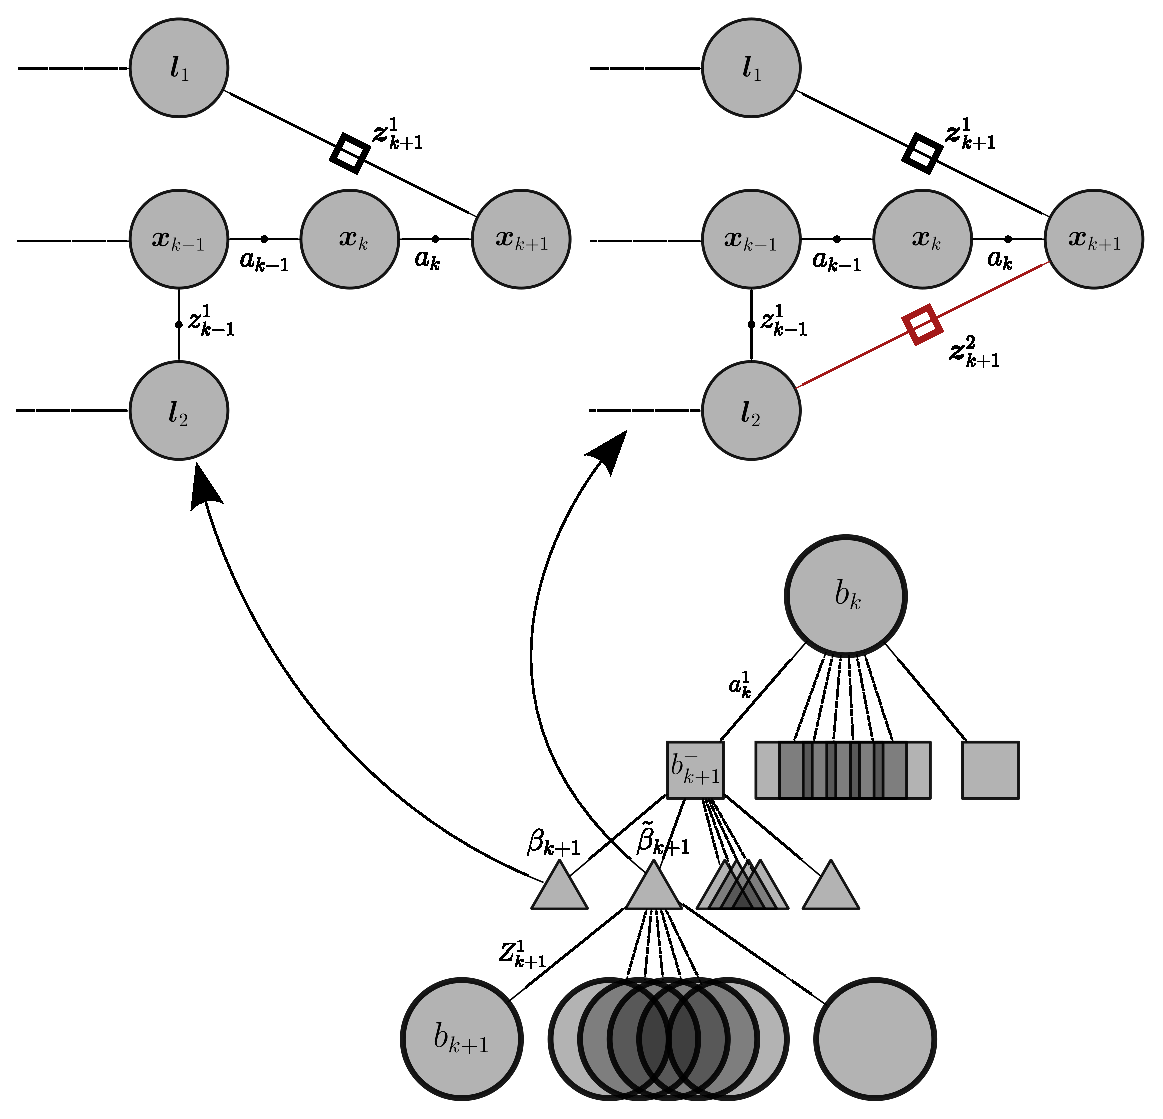
\includegraphics[width=0.4\linewidth,clip]{tree_to_topo.eps}
	\caption{Each da node (triangle) is associated with a specific factor graph topology. At this point the observations associated with the da realizations are still random variables. In the example, by eliminating $\observationRV{k+1}{2}$, the topology resulting from $\tilde{\da{}{}}_{k+1}$ becomes identical to that of $\da{k+1}{}$}
	\label{fig:topology}
\end{figure}
High dimensional problems, such as SLAM, often exhibit structure that allows for the belief to be represented via a factor graph. Planning algorithms that aim to address the problem of high-dimensional planning can thus leverage the topology of the problem as a cheap source of information. The comparison of topology between similar beliefs is captured by the DA variable ($\da{}{}$) as seen in \cref{fig:topology}. We assume that realizations of DA can be generated from the distribution $\probcond{\da{}{}}{\states{}}$ (e.g. a Bernoulli distribution on the failure rate of a locator beacon).

\subsubsection{Complete Factor Elimination}

As illustrated in \cref{fig:topology}, the beliefs of neighboring DA nodes share much of the same topological aspects. More precisely, when $\norm{\da{}{}-\tilde{\da{}{}}}_{1}\ll\abs{L}$ and the history\footnote{When taking into account DA, $\hist{k}\triangleq\{\action{0:k-1},\da{1:k}{},\observations{1:k}\}$} $\priorHist{}$ is shared between the nodes (i.e., they share the same belief-action parent node), then the belief topology is identical up to
$\mathcal{F}\bigl(\abs{\tilde{\da{}{}}-\da{}{}}\bigr)$, where we recall that $f_i\in\mathcal{F}(\da{}{})$ is an observation factor as indicated by $\da{}{i}$. Although in this work we limit our discussion to a myopic comparison of DA, the concept can be extended to a non-myopic form. In the SLAM scenario, $\da{}{}$ encodes the connectivity of pose to landmarks, with the observations yet unspecified (as is symbolized by the square nodes in the factor graphs of \cref{fig:topology}). This similarity in the topology motivates the removal of selected DA nodes, with guarantees in the form of bounds formulated as a function of the remaining DA nodes. We examine \cref{thm:general_bounds} in its application to \eqref{eq:da_bellman} to understand the potential method for eliminating specific realizations of DA.
\begin{equation}
	\label{eq:remove_da}
	\expectation{\expectation{V^\pi(\blf{})}{\observationsRV{}\mid\daRV{}{}}}{\daRV{}{}}-\partialexpectation{\expectation{V^\pi(\blf{})}{\observationsRV{}\mid\daRV{}{}}}{\subSpace}=\sum_{\da{i}{}\in\stcomp{\subSpace}}\measure{\da{i}{}}\expectation{V^\pi(\blf{})}{\observationsRV{}\mid\da{i}{}}\;.
\end{equation}
where $\subSpace\subseteq\mathcal{D}$.

\Cref{eq:remove_da} is an equality as we have not yet bounded the expected value function. The next step is to bound the conditional expectation.

\subsubsection{Application to Conditional Entropy}

For an application of eliminating realizations of DA, we look to conditional entropy as our expected reward. \Cref{thm:entropy_bounds} forms the basis of our bounds, but it does not take into consideration different DAs. This brings us to our novel bound on the conditional entropy that takes advantage of the problem topology in order to make high-dimensional planning more tractable.

\begin{propositionE}[][end, no link to proof]
	\label{thm:entropy_high_dim_bounds}
	The conditional entropy of the random variable $\statesRV{}$ given the random variable $\observationsRV{}=\observationRV{}{1:n}$ can be bounded by the difference of the partial expectation with respect to $\observationRV{}{1:m}$ for $m\leq n$. Thus $\lowerbound_m\leq\condEntropy{\statesRV{}}{\observationsRV{}}-\simplecondEntropy{\statesRV{}}{\observationsRV{}}{m}\leq\upperbound_m$, where:
	\begin{small}
		\begin{subequations}
			\begin{align}
				\lowerbound\nolimits_m & =-\sum_{i=1}^m\measure{\stcompI{\subSpace}{i}}\left(\log\sup_{\observation{}{i}\in\stcompI{\subSpace}{i}}M_{\observation{}{i}}-\log m_{\norm{\observation{}{i}}}(\stcompI{\subSpace}{i})\right)-\upperbound_{\observationRV{}{m+1:n}}\left(\expectation{\log C_{pm}}{\observationsRV{}}\right)\;,
				\\
				\upperbound\nolimits_m  & =-\sum_{i=1}^m\measure{\stcompI{\subSpace}{i}}\left(\log\inf_{\observation{}{i}\in\stcompI{\subSpace}{i}}m_{\observation{}{i}}-\log M_{\norm{\observation{}{i}}}(\stcompI{\subSpace}{i})\right)\;,\\
				\begin{split} \simplecondEntropy{\statesRV{}}{\observationsRV{}}{m}&\triangleq\entropy{\statesRV{}}+\expectation{\log\pnorm{\prod_{j=m+1}^n\probcond{\observationRV{}{j}}{\states{}}\prob{\states{}}}{q}{\states{}}}{\observationRV{}{m+1:n}}                    \\
					&\phantomeq+\sum_{i=1}^m\partialexpectation{\log\pnorm{\probcond{\observationRV{}{i}}{\states{}}}{p}{\states{}}}{\subSpace_i}-\partialexpectation{\expectation{\log\probcond{\observationRV{}{i}}{\statesRV{}}}{\statesRV{}\mid\observationRV{}{i}}}{\subSpace_i}\;,
				\end{split}
			\end{align}
		\end{subequations}
	\end{small}
	and
	\begin{equation}
		\begin{split}
			& \upperbound_{\observationRV{}{1:m}}\left(\expectation{\log C_{pm}}{\observationsRV{}}\right)\\
			& \quad=-\frac{m\log p}{p}-\frac{\log q}{q}\\
			& \quad\phantomeq-\prod_{i=1}^m\measure{\subSpace_i}\Biggl(\expectation{\log m_{\states{}}}{\observationRV{}{m+1:n}}+\sum_{j=1}^m\frac{\partialexpectation{\log m_j}{\subSpace_j}}{\measure{\subSpace_j}}\Biggr) \\
			& \quad\phantomeq+\E_{\observationRV{}{m+1:n}}\Biggl[\partexp_{\subSpace_1}\Biggl[\dotsi\partexp_{\subSpace_m}\Biggl[
			\log \Biggl(\sum_{i=1}^{m} M_{\observation{}{i}}^{p-1}m_{\observation{}{i}}+M_{\states{}}^{q-1}m_{\states{}}\Biggr)\Biggr]\dotsi\Biggr]\Biggr]                                                                    \\
			& \quad\phantomeq+\left(1-\prod_{i=1}^m\measure{\subSpace_i}\right)\Biggl(-\sum_{i=1}^m\log \inf m_{\observation{}{i}}\\
			& \quad\quad\phantomeq+\E_{\observationRV{}{m+1:n}}\left[-\log m_{\states{}}+\log\left(\sum_{i=1}^{m}\left(\sup M_{\observation{}{i}}\right)^{p-1}\inf m_{\observation{}{i}} +M_{\states{}}^{q-1}m_{\states{}}\right)\right]\Biggr)
		\end{split}
	\end{equation}
\end{propositionE}
\begin{proofE}
	$\condEntropy{\observationsRV{}}{\statesRV{}}=\sum\limits_{i=1}^{\abs{\observationsRV{}}}\condEntropy{\observationRV{}{i}}{\statesRV{}}$ assuming conditional independence of the observations, as such we can bound $\condEntropy{\observationsRV{}}{\statesRV{}}$ with a sum of bounds from \cref{thm:observation_bounds}.
\end{proofE}

\begin{propositionE}[][end, no link to proof]
	\label{thm:normalizer_bounds_struct}
	$\lowerbound_m\leq\entropy{\observationsRV{}} -\simplentropy{\observationsRV{}}{m}\leq\upperbound_m$ for $\observationsRV{}=\observationRV{}{1:n}$, where:
	\begin{subequations}
		\begin{align}
			\lowerbound\nolimits_m & =-\sum_{i=1}^m\measure{\stcompI{\subSpace}{i}}\log M_{\norm{\observation{}{i}}}(\stcompI{\subSpace}{i})\;, \\
			\upperbound\nolimits_m & =-\sum_{i=1}^m\measure{\stcompI{\subSpace}{i}}\log m_{\norm{\observation{}{i}}}(\stcompI{\subSpace}{i})+\upperbound_{\observationRV{}{1:m}}\left(\expectation{\log C_{pm}}{\observationsRV{}}\right)\;,\\
			\begin{split}
				\simplentropy{\observationsRV{}}{m} & \triangleq-\sum_{i=1}^m\partialexpectation{\log\pnorm{\probcond{\observationRV{}{i}}{\states{}}}{p}{\states{}}}{\subSpace_i}\\
				&\phantomeq-\expectation{\log\pnorm{\prod_{j=m+1}^n\probcond{\observationRV{}{j}}{\states{}}\prob{\states{}}}{q}{\states{}}}{\observationRV{}{m+1:n}}\;,
			\end{split}
		\end{align}
	\end{subequations}
	and
	\begin{equation}
		\begin{split}
			& \upperbound_{\observationRV{}{1:m}}\left(\expectation{\log C_{pm}}{\observationsRV{}}\right)\\
			& \quad=-\frac{m\log p}{p}-\frac{\log q}{q}
			-\prod_{i=1}^m\measure{\subSpace_i}\Biggl(\expectation{\log m_{\states{}}}{\observationRV{}{m+1:n}}+\sum_{j=1}^m\frac{\partialexpectation{\log m_j}{\subSpace_j}}{\measure{\subSpace_j}}\Biggr) \\
			& \quad\phantomeq+\E_{\observationRV{}{m+1:n}}\Biggl[\partexp_{\subSpace_1}\Biggl[\dotsi\partexp_{\subSpace_m}\Biggl[
			\log \Biggl(\sum_{i=1}^{m} M_{\observation{}{i}}^{p-1}m_{\observation{}{i}}
			+M_{\states{}}^{q-1}m_{\states{}}\Biggr)\Biggr]\dotsi\Biggr]\Biggr]\\
			& \quad\phantomeq+\left(1-\prod_{i=1}^m\measure{\subSpace_i}\right)\Biggl(-\sum_{i=1}^m\log \inf m_{\observation{}{i}}\\
			& \quad\phantomeq+\E_{\observationRV{}{m+1:n}}\Bigl[-\log m_{\states{}}
			+\log\Bigl(\sum_{i=1}^{m}\left(\sup M_{\observation{}{i}}\right)^{p-1}\inf m_{\observation{}{i}}+M_{\states{}}^{q-1}m_{\states{}}\Bigr)\Bigr]\Biggr)
		\end{split}
	\end{equation}
\end{propositionE}
\begin{proofE}
	For both bounds we begin by bounding the normalizer,
	\begin{equation*}
		\begin{split}
			\prob{\observationsRV{}} & =\int\probcond{\observationRV{}{1:n}}{\states{}}\prob{\states{}}\D\states{}\\
			& =\int\prod_{i=1}^n\probcond{\observationRV{}{i}}{\states{}}\prob{\states{}}\D\states{}
		\end{split}
	\end{equation*}
	above by
	\begin{equation}
		\prob{\observationsRV{}}\leq\prod_{i=1}^{m}\pnorm{\probcond{\observationRV{}{i}}{\states{}}}{p}{\states{}}\pnorm{\prod_{j=m+1}^n\probcond{\observationRV{}{j}}{\states{}}\prob{\states{}}}{q}{\states{}}
		\label{eq:holders}
	\end{equation}
	and below by (see~\cite{Wang77cmb})
	\begin{equation}
		\prob{\observationsRV{}}\geq C_{pm}^{-1}\prod_{i=1}^{m}\pnorm{\probcond{\observationRV{}{i}}{\states{}}}{p}{\states{}}\pnorm{\prod_{j=m+1}^n\probcond{\observationRV{}{j}}{\states{}}\prob{\states{}}}{q}{\states{}}\label{eq:reverse_holders}
	\end{equation}
	where $p=\frac{mq}{q-1}$ and
	\begin{align*}
		&C_{pm}\triangleq\frac{\sum_{i=1}^{m} K_i(p)+K_{m+1}(q)}{p^{m/p}q^{1/q}},\\
		&K_i(p)\triangleq\frac{M_{\observation{}{i}}^{p-1}}{\displaystyle m_{\states{}}\prod_{k\neq i}m_k},&&
		K_{m+1}(q)\triangleq\frac{M_{\states{}}^{q-1}}{\displaystyle\prod_{k}m_{\observation{i}{}}},\\
		&M_{\observation{i}{}}\triangleq\sup_{\states{}}\probcond{\observationRV{i}{}}{\states{}},&&
		m_{\observation{i}{}}\triangleq\inf_{\states{}}\probcond{\observationRV{i}{}}{\states{}},
		\\
		&M_{\states{}}\triangleq\sup_{\states{}}\prod_{j=m+1}^n\probcond{\observationRV{}{j}}{\states{}}\prob{\states{}},&&
		m_{\states{}}\triangleq\inf_{\states{}}\prod_{j=m+1}^n\probcond{\observationRV{}{j}}{\states{}}\prob{\states{}},
	\end{align*}
	under the assumption that the infimum of the functions is greater than zero.

	In the following we will prove the upper bound, the lower bound is derived in a similar manner but for $C_{pm}=1$. Applying inequalities \eqref{eq:reverse_holders}, and proposition \eqref{thm:bound_log} we find that entropy of the normalizer is bounded above
	\begin{small}
		\begin{align}
			\begin{split}
				\entropy{\observationsRV{}} & \leq\expectation{\log C_{pm}}{\observationRV{}{1:n}}
				-\expectation{\sum_{i=1}^{m}\log\left(\pnorm{\probcond{\observationRV{}{i}}{\states{}}}{p}{\states{}}\right)}{\observationRV{}{1:n}}\\
				&\phantomeq-\expectation{\log\pnorm{\prod_{j=m+1}^n\probcond{\observationRV{}{j}}{\states{}}\prob{\states{}}}{q}{\states{}}}{\observationRV{}{1:n}}
			\end{split}\\
			\begin{split}
				& =\expectation{\log C_{pm}}{\observationRV{}{1:n}}
				-\sum_{i=1}^{m}\expectation{\log\left(\pnorm{\probcond{\observationRV{}{i}}{\states{}}}{p}{\states{}}\right)}{\observationRV{}{i}}\\
				&\phantomeq-\expectation{\log\pnorm{\prod_{j=m+1}^n\probcond{\observationRV{}{j}}{\states{}}\prob{\states{}}}{q}{\states{}}}{\observationRV{}{m+1:n}}
			\end{split}\\
			\begin{split}
				& \leq\expectation{\log C_{pm}}{\observationRV{}{1:n}}
				-\sum_{i=1}^{m}\partialexpectation{\log\left(\pnorm{\probcond{\observationRV{}{i}}{\states{}}}{p}{\states{}}\right)}{\subSpace_i}\\
				&\phantomeq-\sum_{i=1}^{m}\measure{\stcompI{\subSpace}{i}}\inf_{\observation{}{i}\in\subSpace_i}\log\left(\pnorm{\probcond{\observation{}{i}}{\states{}}}{p}{\states{}}\right) \\
				&\phantomeq-\expectation{\log\pnorm{\prod_{j=m+1}^n\probcond{\observationRV{}{j}}{\states{}}\prob{\states{}}}{q}{\states{}}}{\observationRV{}{m+1:n}}
			\end{split} \\
			\begin{split}
				& \leq\expectation{\log C_{pm}}{\observationRV{}{1:n}}-\sum_{i=1}^{m}\partialexpectation{\log\left(\pnorm{\probcond{\observationRV{}{i}}{\states{}}}{p}{\states{}}\right)}{\subSpace_i}\\
				& \phantomeq-\sum_{i=1}^{m}\measure{\stcompI{\subSpace}{i}}\log m_{\norm{\observation{}{i}}}(\stcompI{\subSpace}{i})-\expectation{\log\pnorm{\prod_{j=m+1}^n\probcond{\observationRV{}{j}}{\states{}}\prob{\states{}}}{q}{\states{}}}{\observationRV{}{m+1:n}}
			\end{split}
		\end{align}
	\end{small}
	Via the definition of $C_{pm}$ we can further refine the bound
	\begin{align*}
		\expectation{\log C_{pm}}{\observationRV{}{1:n}} & =-\frac{m\log p}{p}-\frac{\log q}{q}+\expectation{\log\frac{\sum_{i=1}^{m} M_{\observation{}{i}}^{p-1}m_{\observation{}{i}}+M_{\states{}}^{q-1}m_{\states{}}}{m_{\states{}}\prod_{i=1}^{m}m_{\observation{}{i}}}}{\observationRV{}{1:n}}\\
		\begin{split}
			& \leq-\frac{m\log p}{p}-\frac{\log q}{q}\\
			& \phantomeq+\E_{\observationRV{}{m+1:n}}\Biggl[\partexp_{\subSpace_1\times\cdots\times\subSpace_m}\Biggl[
			\log\frac{\sum_{i=1}^{m}M_{\observation{}{i}}^{p-1}m_{\observation{}{i}}+M_{\states{}}^{q-1}m_{\states{}}}{m_{\states{}}\prod_{i=1}^{m}m_{\observation{}{i}}}\Biggr] \\
			&\phantomeq
			+\left(1-\prod_{i=1}^m\measure{\subSpace_i}\right)\sup_{\observation{}{1:m}\in\stcomp{{\left(\subSpace_1\times\cdots\times\subSpace_m\right)}}}
			\log\frac{\sum_{i=1}^{m} M_{\observation{}{i}}^{p-1}m_{\observation{}{i}}+M_{\states{}}^{q-1}m_{\states{}}}{m_{\states{}}\prod_{i=1}^{m}m_{\observation{}{i}}}\Biggr]
		\end{split}\\
		\begin{split}
			& \leq-\frac{m\log p}{p}-\frac{\log q}{q}\\
			& \phantomeq
			-\prod_{i=1}^m\measure{\subSpace_i}\Biggl(\expectation{\log m_{\states{}}}{\observationRV{}{m+1:n}}
			+\sum_{j=1}^m\frac{\partialexpectation{\log m_j}{\subSpace_j}}{\measure{\subSpace_j}}\Biggr)          \\
			& \phantomeq
			+\E_{\observationRV{}{m+1:n}}\Biggl[\partexp_{\subSpace_1}\Biggl[\dotsi\partexp_{\subSpace_m}\Biggl[
			\log \Biggl(\sum_{i=1}^{m} M_{\observation{}{i}}^{p-1}m_{\observation{}{i}}
			+M_{\states{}}^{q-1}m_{\states{}}\Biggr)\Biggr]\dotsi\Biggr]\Biggr]                                   \\
			& \phantomeq
			+\left(1-\prod_{i=1}^m\measure{\subSpace_i}\right)\Biggl(-\sum_{i=1}^m\log \inf m_{\observation{}{i}} \\
			& \phantomeq
			+\E_{\observationRV{}{m+1:n}}\Bigl[-\log m_{\states{}}
			+\log\Bigl(\sum_{i=1}^{m}\left(\sup M_{\observation{}{i}}\right)^{p-1}\inf m_{\observation{}{i}}
			+M_{\states{}}^{q-1}m_{\states{}}\Bigr)\Bigr]\Biggr)
		\end{split}
	\end{align*}
\end{proofE}
\OLO{we use the conditional independence between observations.}
Note that $m_{\norm{\observation{}{i}}}(\subSpace)\geq \inf\limits_{\observation{}{i}\in\subSpace}m_{\observation{}{i}}$ and $M_{\norm{\observation{}{i}}}(\subSpace)\leq \sup\limits_{\observation{}{i}\in\subSpace}M_{\observation{}{i}}$ and can be used to loosen the bounds if needed.

\begin{corollaryE}[][end, no link to proof]
	\label{thm:bounds_elim}
	$\lowerbound(\da{\textup{diff}}{})\leq\condEntropy{\statesRV{}}{\observationsRV{},\tilde{\da{}{}}}-\simplecondEntropy{\statesRV{}}{\observationsRV{},\da{}{},\tilde{\da{}{}}}{}\leq\upperbound(\da{}{},\tilde{\da{}{}})\quad\forall\tilde{\da{}{}},\da{}{}\in\mathcal{D}$, where:
	\begin{small}
		\begin{subequations}
			\begin{align}
				\lowerbound(\da{}{},\tilde{\da{}{}}) & =-\sum_{f_i\in\mathcal{F}(\da{\textup{diff}}{})}\left(\log\sup M_{f_i}-\log m_{\norm{f_i}}\right)-\upperbound_{\da{}{\prime}}\Bigl(\expectation{\log C_{pm}}{\observationsRV{}}\Bigr)\;,\\
				\upperbound(\da{\textup{diff}}{}) & =-\sum_{f_i\in\mathcal{F}(\da{\textup{diff}}{})}\left(\log\inf m_{f_i}-\log M_{\norm{f_i}}\right)\;,\\
				\simplecondEntropy{\statesRV{}}{\observationsRV{},\da{}{},\tilde{\da{}{}}}{}&\triangleq\entropy{\statesRV{}} +\E_{\observationsRV{}{}\mid\da{}{\prime}}\Biggl[{\log\Big\lVert{\prob{\states{}}\prod_{f_i\in\mathcal{F}(\da{}{\prime})}f_i}\Big\rVert_{q}^{\states{}}}\Biggr]\;,
			\end{align}
		\end{subequations}
	\end{small}
	$\da{\textup{diff}}{i}\triangleq\max(\tilde{\da{}{i}}-\da{}{i},0)$, $\da{}{\prime}\triangleq\tilde{\da{}{}}-\da{\textup{diff}}{}$ and	$\upperbound_{\da{}{\prime}}\Bigl(\expectation{\log C_{pm}}{\observationsRV{}}\Bigr)$ is defined in the proof.
\end{corollaryE}
\begin{proofE}
	From \cref{thm:entropy_high_dim_bounds}, if we take the global extremes and completely eliminate the observations we trivially arrive at the desired statement.

	For this case:
	\begin{equation*}
		\begin{split}
			\upperbound_{\da{}{\prime}}\left(\expectation{\log C_{pm}}{\observationsRV{}}\right)&=-\frac{m\log p}{p}-\frac{\log q}{q}-\sum_{f_i\in\mathcal{F}(\da{\textup{diff}}{})}\log \inf m_{f_i}-\expectation{\log m_{\states{}}}{\observationsRV{}{}\mid\da{}{\prime}}\\
			&\phantomeq+\E_{\observationsRV{}{}\mid\da{}{\prime}}\left[\log\left(\sum_{f_i\in\mathcal{F}(\da{\textup{diff}}{})}\left(\sup M_{f_i}\right)^{p-1}\inf m_{f_i}+M_{\states{}}^{q-1}m_{\states{}}\right)\right]\;,
		\end{split}
	\end{equation*}
	where
	\begin{align*}
		&M_{f_i}\triangleq\sup_{\states{}}\probcond{\observationRV{i}{}}{\states{}}\;,&&
		m_{f_i}\triangleq\inf_{\states{}}\probcond{\observationRV{i}{}}{\states{}}\;,
		\\
		&M_{\states{}}\triangleq\sup_{\states{}}\prod_{f_i\in\mathcal{F}(\da{}{\prime})}f_i\prob{\states{}}\;,&&
		m_{\states{}}\triangleq\inf_{\states{}}\prod_{f_i\in\mathcal{F}(\da{}{\prime})}f_i\prob{\states{}}\;.
	\end{align*}
\end{proofE}

It should be noted that for the bounds to be meaningful, $\inf m_{f_i}>0$. For example, this is not the case when $f_i$ is the Gaussian distribution. Furthermore, this limits the discussion of $f_i$ to finite support.

As an example let us assume $\tilde{\da{}{}}=\begin{bmatrix}1&1&0\end{bmatrix}^\intercal$ and $\da{}{}=\begin{bmatrix}0&1&1\end{bmatrix}^\intercal$. For such a case we find that $\da{\textup{diff}}{}=\begin{bmatrix}1&0&0\end{bmatrix}^\intercal$ and $\da{}{\prime}=\begin{bmatrix}0&1&0\end{bmatrix}^\intercal$. We note that $\da{}{\prime}$ indicates as to what associations are shared between $\tilde{\da{}{}}$ and $\da{}{}$. We provide the equivalent definitions $\da{}{i\prime}\equiv \tilde{\da{}{i}}\land\da{}{i}$ and $\da{\textup{diff}}{i}\equiv \tilde{\da{}{i}}\land\lnot\da{}{i}$.
When $\tilde{\da{}{}}\succeq\da{}{}$, $\da{}{\prime}\equiv\da{}{}$ and when $\tilde{\da{}{}}\preceq\da{}{}$, $\da{\textup{diff}}{}=0$ resulting in no computational benefit, as the computational benefit is proportional to $\norm{\da{\textup{diff}}{}}_1$. This highlights the trade-off between computational efficiency and tightness of the bounds when selecting a $\da{}{}\in\subSpace$ for the computation of \cref{thm:bounds_elim}.

To incorporate \cref{thm:bounds_elim} into planning, the bounds must be applied in the context of the value function. As shown, the bounds are myopic and bound the immediate expected reward. \Cref{thm:val_func_immediate_bounds_obs_bellman} allows for bounding the value function with respect to bounds on the immediate expected reward. In a similar fashion we can bound the expected value function as shown in \eqref{eq:remove_da}, where now different realizations of DA are taken into consideration.

We are unaware of prior works that provide bounds on the value function while considering different DA realizations, when the reward is the entropy of the state. In~\cite{Shienman22icra} the authors consider the Shannon entropy of the hypothesis probabilities. In~\cite{Yotam24tro} the authors consider simplification of the observation space for the expected differential entropy for a given DA.